\documentclass[12pt,a4paper]{article}

\usepackage[a4paper,text={16.5cm,25.2cm},centering]{geometry}
\usepackage{lmodern}
\usepackage{amssymb,amsmath}
\usepackage{bm}
\usepackage{graphicx}
\usepackage{microtype}
\usepackage{hyperref}
\usepackage{minted}
\setlength{\parindent}{0pt}
\setlength{\parskip}{1.2ex}

\hypersetup
       {   pdfauthor = {  },
           pdftitle={  },
           colorlinks=TRUE,
           linkcolor=black,
           citecolor=blue,
           urlcolor=blue
       }






\begin{document}



\section{Robni problem za Laplaceovo enačbo}

\begin{minted}[texcomments = true, mathescape, fontsize=\small, xleftmargin=0.5em]{julia}
using Vaje04

rp = Vaje04.RobniProblemPravokotnikLaplace(
    [0,pi,-1,1],
    [sin, sin ,x->0.0 ,x->0.0]
)
\end{minted}
\begin{minted}[texcomments = true, mathescape, fontsize=\small, xleftmargin=0.5em, frame = leftline]{text}
RobniProblemPravokotnikLaplace([0.0, 3.141592653589793, -1.0, 1.0], Functio
n[sin, sin, Main.var"##WeaveSandBox#231".var"#1#3"(), Main.var"##WeaveSandB
ox#231".var"#2#4"()])
\end{minted}

funkcija resi ne deluje kot pričakovano


\begin{minted}[texcomments = true, mathescape, fontsize=\small, xleftmargin=0.5em]{julia}
Z = resi(rp,0.1)


using Plots
surface(Z)
\end{minted}
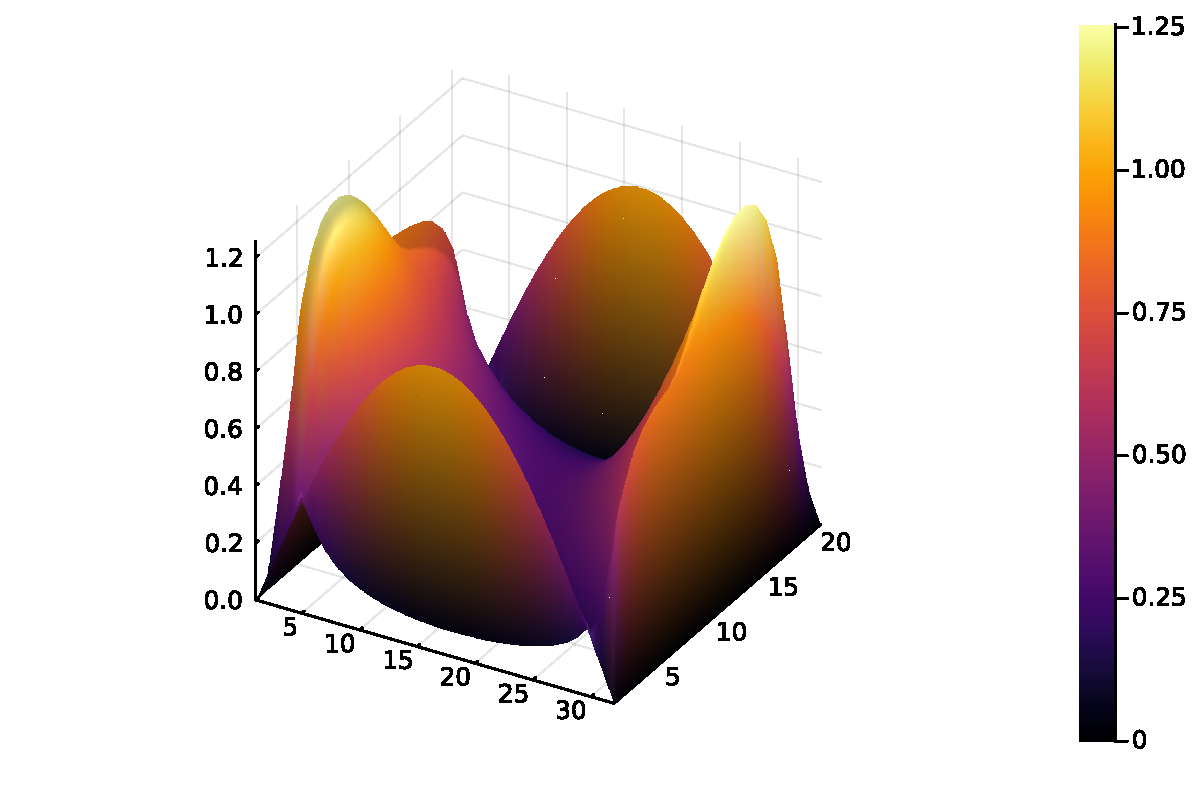
\includegraphics[width=\linewidth]{jl_LvC1bB/demo_2_1.pdf}

Narisana ploskev


Napolnitev Laplaceove matrike


\begin{minted}[texcomments = true, mathescape, fontsize=\small, xleftmargin=0.5em]{julia}
L = laplaceova_matrika(10,10)
spy(L)

using LinearAlgebra
\end{minted}

Obzervacija - na nediagonalnih mestih neničelni elementi


\begin{minted}[texcomments = true, mathescape, fontsize=\small, xleftmargin=0.5em]{julia}
F = lu(L)
spy(F.L)

spy(F.U)
\end{minted}
\includegraphics[width=\linewidth]{jl_LvC1bB/demo_4_1.pdf}

\section{Iterativne metode}

\begin{minted}[texcomments = true, mathescape, fontsize=\small, xleftmargin=0.5em]{julia}
Z = resi_iter(rp,0.1,1) #Gauss-Seidlova iteracija
surface(Z)
\end{minted}
\begin{minted}[texcomments = true, mathescape, fontsize=\small, xleftmargin=0.5em, frame = leftline]{text}
Število iteracij: 566
\end{minted}
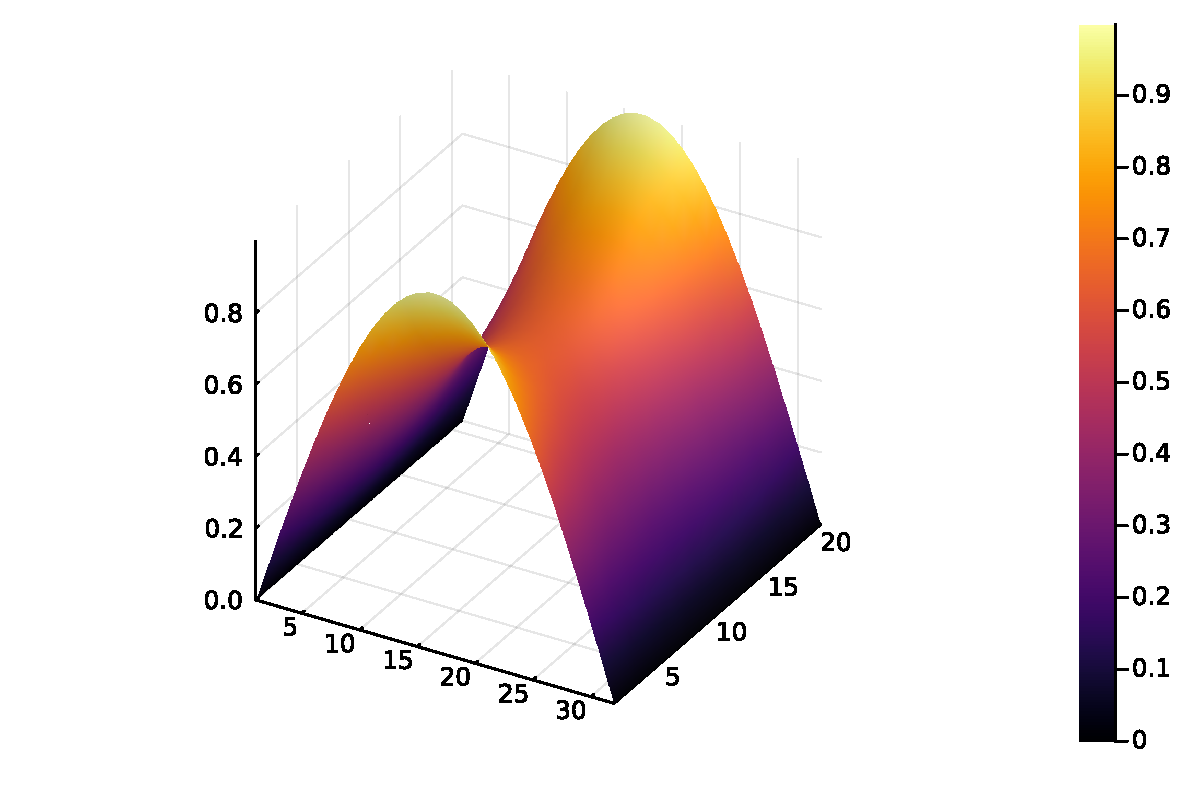
\includegraphics[width=\linewidth]{jl_LvC1bB/demo_5_1.pdf}

Naslednji graf


\begin{minted}[texcomments = true, mathescape, fontsize=\small, xleftmargin=0.5em]{julia}
resi_iter(rp,0.1,1.5)
\end{minted}
\begin{minted}[texcomments = true, mathescape, fontsize=\small, xleftmargin=0.5em, frame = leftline]{text}
Število iteracij: 205
21|$\ensuremath{\times}$|32 Matrix{Float64}:
 0.0  0.101168   0.201299  0.299363  |$\ensuremath{\ldots}$|  0.299363  0.201299  0.101168   0.0
 0.0  0.0938184  0.186674  0.277614     0.277615  0.186675  0.0938187  0.0
 0.0  0.0874313  0.173965  0.258715     0.258716  0.173966  0.0874317  0.0
 0.0  0.0819414  0.163042  0.24247      0.242471  0.163043  0.081942   0.0
 0.0  0.0772923  0.153792  0.228713     0.228715  0.153793  0.0772931  0.0
 0.0  0.0734365  0.146119  0.217303  |$\ensuremath{\ldots}$|  0.217305  0.146121  0.0734374  0.0
 0.0  0.0703343  0.139947  0.208124     0.208126  0.139949  0.0703353  0.0
 0.0  0.0679538  0.13521   0.20108      0.201082  0.135212  0.0679549  0.0
 0.0  0.0662708  0.131862  0.1961       0.196102  0.131864  0.0662719  0.0
 0.0  0.0652678  0.129866  0.193132     0.193135  0.129868  0.065269   0.0
 |$\ensuremath{\vdots}$|                                   |$\ensuremath{\ddots}$|                      |$\ensuremath{\vdots}$|          
 0.0  0.066271   0.131862  0.1961       0.196103  0.131864  0.066272   0.0
 0.0  0.0679541  0.135211  0.201081     0.201083  0.135213  0.067955   0.0
 0.0  0.0703346  0.139948  0.208125     0.208127  0.139949  0.0703354  0.0
 0.0  0.0734369  0.14612   0.217304  |$\ensuremath{\ldots}$|  0.217306  0.146122  0.0734376  0.0
 0.0  0.0772927  0.153792  0.228714     0.228715  0.153793  0.0772933  0.0
 0.0  0.0819417  0.163043  0.242471     0.242472  0.163043  0.0819421  0.0
 0.0  0.0874316  0.173966  0.258715     0.258716  0.173967  0.0874319  0.0
 0.0  0.0938186  0.186675  0.277615     0.277615  0.186675  0.0938187  0.0
 0.0  0.101168   0.201299  0.299363  |$\ensuremath{\ldots}$|  0.299363  0.201299  0.101168   0.0
\end{minted}


\end{document}
